\documentclass[12pt, a4paper]{article}

% ── Paquetes ──────────────────────────────────────────────────────────────────
\usepackage[utf8]{inputenc}
\usepackage[T1]{fontenc}
\usepackage[spanish]{babel}
\usepackage{geometry}
\usepackage{setspace}
\usepackage{graphicx}
\usepackage{float}
\usepackage{booktabs}
\usepackage{longtable}
\usepackage{array}
\usepackage{hyperref}
\usepackage{url}
\usepackage{amsmath}
\usepackage{caption}
\usepackage{subcaption}
\usepackage{fancyhdr}
\usepackage{titlesec}
\usepackage{parskip}
\usepackage{multirow}
\usepackage{tabularx}
\usepackage[table]{xcolor}
\usepackage{tcolorbox}
\tcbuselibrary{skins,breakable}
\usepackage{mdframed}
\usepackage{tikz}
\usepackage{lmodern}
\usepackage{microtype}
\usepackage{colortbl}
\usepackage{multicol}
\usepackage{needspace}
\usepackage{placeins}

% ── Colores principales ───────────────────────────────────────────────────────
\definecolor{primary}{RGB}{13, 71, 161}       % Azul oscuro (satélite/espacio)
\definecolor{secondary}{RGB}{2, 136, 209}     % Azul medio
\definecolor{accent}{RGB}{0, 188, 212}        % Cyan (teledetección)
\definecolor{lightbg}{RGB}{232, 244, 253}     % Azul muy claro (fondo)
\definecolor{darktext}{RGB}{30, 30, 30}
\definecolor{tableheader}{RGB}{13, 71, 161}
\definecolor{tablerow}{RGB}{232, 244, 253}

\setlength{\columnsep}{0.6cm}
\setlength{\columnseprule}{0.4pt}
\def\columnseprulecolor{\color{accent}}

% ── Márgenes de portada (se cambian a márgenes del cuerpo tras la portada) ───
\geometry{
    top=1.5cm,
    bottom=1.5cm,
    left=1.5cm,
    right=1.5cm,
    headheight=15pt,
    headsep=0.5cm
}

\onehalfspacing

% Evitar líneas viudas y huérfanas
\widowpenalty=10000
\clubpenalty=10000

% ── Estilo de secciones ───────────────────────────────────────────────────────
\titleformat{\section}
  {\color{primary}\large\bfseries}
  {\color{accent}\thesection.}{0.5em}{}
  [\color{secondary}\titlerule]

\titleformat{\subsection}
  {\color{secondary}\normalsize\bfseries}
  {\thesubsection.}{0.5em}{}

\titleformat{\subsubsection}
  {\color{darktext}\normalsize\itshape}
  {\thesubsubsection.}{0.5em}{}

\titlespacing{\section}{0pt}{14pt}{6pt}
\titlespacing{\subsection}{0pt}{10pt}{4pt}

% ── Encabezado y pie de página ────────────────────────────────────────────────
\pagestyle{fancy}
\fancyhf{}
\renewcommand{\headrulewidth}{2pt}
\renewcommand{\headrule}{\color{primary}\hrule width\headwidth height 2pt \vspace{1pt}\color{accent}\hrule width\headwidth height 1pt}
\fancyhead[L]{\color{primary}\small\textbf{Análisis Geoespacial en el Conflicto Rusia-Ucrania}}
\fancyhead[R]{\color{primary}\small D. Silva Madariaga \quad \textbf{\thepage}}

% ── Hipervínculos ─────────────────────────────────────────────────────────────
\hypersetup{
    colorlinks=true,
    linkcolor=primary,
    citecolor=secondary,
    urlcolor=secondary
}

% ── Bibliografía sin números (formato APA) ────────────────────────────────────
\makeatletter
\renewcommand\@biblabel[1]{}
\makeatother

% ── Caption style ─────────────────────────────────────────────────────────────
\captionsetup{
    font=small,
    labelfont={bf, color=primary},
    labelsep=period
}

% ──────────────────────────────────────────────────────────────────────────────
\begin{document}
\color{darktext}
\singlespacing   % Espaciado simple en portada para evitar desbordamiento

% ══════════════════════════════════════════════════════════════════════════════
% PORTADA
% ══════════════════════════════════════════════════════════════════════════════
\thispagestyle{empty}
\pagenumbering{roman}
\setcounter{page}{1}

% ── Layout de dos columnas tipo revista ───────────────────────────────────────
\noindent
\begin{minipage}[t]{0.63\textwidth}

  % Caja azul con título
  \begin{tcolorbox}[
      colback=primary,
      colframe=primary,
      arc=0pt,
      boxrule=0pt,
      left=10pt, right=10pt, top=14pt, bottom=14pt,
      width=\textwidth
  ]
    {\fontsize{18}{24}\selectfont\bfseries\color{white}
    Análisis Geoespacial Aplicado al\\[0.3cm]
    Conflicto Rusia-Ucrania:\\[0.3cm]
    Revisión Bibliométrica\\[0.3cm]
    \par}
  \end{tcolorbox}

  \vspace{0.4cm}

  % Autor
  {\color{primary}\bfseries\small DIEGO ERNESTO SILVA MADARIAGA}\\[0.1cm]
  {\color{darktext}\footnotesize Universidad Tecnológica Metropolitana, Facultad de Ingeniería,\\
  Ingeniería Civil en Ciencia de Datos, Santiago, Chile.}\\[0.1cm]
  {\color{secondary}\footnotesize\itshape diego.silva.12a@gmail.com}

  \vspace{0.4cm}
  {\color{accent}\rule{\textwidth}{0.8pt}}
  \vspace{0.3cm}

  % Abstract
  {\color{primary}\bfseries\small ABSTRACT}

  \vspace{0.2cm}
  {\small El conflicto armado entre Rusia y Ucrania iniciado en febrero de 2022, ha generado una creciente demanda de métodos objetivos y seguros para evaluar los impactos territoriales, ambientales y humanitarios. El análisis geoespacial mediante teledetección satelital ha emergido como la herramienta central para responder a esta necesidad. Esta investigacion constituye una revisión bibliométrica cuyo objetivo es sistematizar y analizar el estado del arte de las metodologías de análisis geoespacial aplicadas al conflicto ruso-ucraniano. Siguiendo los lineamientos PRISMA, se realizó una búsqueda sistemática en las bases de datos Web of Science y Scopus, obteniendo 36 artículos para el análisis final. Los resultados evidencian una amplia diversidad de técnicas, con predominio de imágenes SAR (Sentinel-1), sensores ópticos (Sentinel-2, Landsat) y datos de luz nocturna (VIIRS), aplicadas al monitoreo de impactos agrícolas, urbanos y ambientales en las regiones orientales y meridionales de Ucrania. Se identifican como principales brechas la escasez de validación y la limitada integración de fuentes de datos no convencionales. Como trabajo futuro, se propone la aplicación de algoritmos de clustering espacial como K-Means para la identificación de zonas de concentración de bombardeos y principales puntos calientes del frente.}

  \vspace{0.3cm}
  {\color{accent}\rule{\textwidth}{0.8pt}}

\end{minipage}
\hfill
% ── Columna derecha ───────────────────────────────────────────────────────────
\begin{minipage}[t]{0.33\textwidth}

  \begin{center}
    
\includegraphics[width=0.7\textwidth]{Logo-UTEM-1.png}
  \end{center}

  \vspace{0.4cm}

  \vspace{0.25cm}
  {\color{primary}\bfseries\footnotesize ASIGNATURA:}\\
  {\footnotesize Metodología de Investigación para Ciencia de Datos}

  \vspace{0.25cm}
  {\color{primary}\bfseries\footnotesize SEMESTRE:}\\
  {\footnotesize Primer Semestre 2026}

  \vspace{0.25cm}
  {\color{accent}\rule{\textwidth}{0.8pt}}
  \vspace{0.15cm}

  {\color{primary}\bfseries\footnotesize PALABRAS CLAVE:}\\
  {\footnotesize análisis geoespacial · teledetección · conflicto armado · Ucrania · revisión de alcance · bibliometría}

  \vspace{0.25cm}
  {\color{accent}\rule{\textwidth}{0.8pt}}
  \vspace{0.15cm}

  {\color{primary}\bfseries\footnotesize HERRAMIENTAS UTILIZADAS:}\\
  {\footnotesize PRISMA 2020 · Scopus · Web of Science · pybibx · NotebookLM}

  \vspace{0.2cm}
  {\color{primary}\bfseries\footnotesize CORPUS ANALIZADO:}\\
  {\footnotesize 36 artículos (Scopus + WoS)}

\end{minipage}

% \newgeometry hace su propio \clearpage internamente → termina portada sin página en blanco
\newgeometry{top=2.5cm, bottom=2cm, left=2.2cm, right=2.2cm, headheight=15pt, headsep=0.6cm}
\onehalfspacing  % Restaurar espaciado 1.5 para el cuerpo

% ══════════════════════════════════════════════════════════════════════════════
% TABLA DE CONTENIDOS
% ══════════════════════════════════════════════════════════════════════════════
\thispagestyle{fancy}
\tableofcontents
\clearpage

% Reiniciar numeración arábiga para el cuerpo
\pagenumbering{arabic}
\setcounter{page}{1}

% ══════════════════════════════════════════════════════════════════════════════
\section{Introducción}
% ══════════════════════════════════════════════════════════════════════════════

\begin{multicols}{2}

La invasión a gran escala de Rusia sobre Ucrania iniciada el 24 de febrero de 2022, desencadenó una de las crisis humanitarias y ambientales más severas del siglo XXI. La presencia de combates activos, territorios ocupados y zonas minadas hizo inviable la recolección de datos mediante métodos convencionales de campo.

Las cifras derivadas del análisis satelital ilustran la escala del impacto: entre 2.34 y 2.40 millones de hectáreas agrícolas fueron abandonadas (Wagner et al., 2025; Li et al., 2026); se mapearon 264 km² de daño urbano abarcando más de 2,288 asentamientos (Scher \& Van Den Hoek, 2025); la intensidad lumínica nocturna cayó entre 81.2\% y 84.0\% a nivel nacional (Wang et al., 2024; Lin et al., 2024); y más de 6.33 millones de personas, el 14\% de la población fueron forzadas al exilio (Guo et al., 2025).

El análisis geoespacial satelital es la respuesta metodológica a esa restricción, permite documentar desde órbita lo que no puede verificarse sobre el terreno. Su aplicación a escala nacional, con más de 17,000 asentamientos monitoreados simultáneamente, fue viable gracias a herramientas de Ciencia de Datos como  machine Learning, procesamiento distribuido en la nube y fusión de datos multisensor (Scher \& Van Den Hoek, 2025; Huang et al., 2023). El conflicto tiene además una dimensión global directa, pues Ucrania produce el 10\% del trigo mundial y exporta más del 50\% del aceite de girasol consumido internacionalmente (Qiu et al., 2026; Wagner et al., 2025).

Pese al volumen creciente de publicaciones desde 2022, ningún trabajo había sintetizado estas metodologías de forma sistemática. Este estudio cubre esa laguna mediante una revisión análisis bibliométrico.

\subsection{Pregunta de Investigación y objetivos}

¿Qué metodologías de análisis geoespacial han sido aplicadas para estudiar los impactos del conflicto ruso-ucraniano, y cuáles son sus principales hallazgos, limitaciones y proyecciones futuras?

\textbf{General:} Sistematizar el estado del arte de las metodologías de análisis geoespacial aplicadas al conflicto Rusia-Ucrania mediante la revisión bibliométrica.

\textbf{Específicos:} Identificar los métodos y tecnologías satelitales más utilizados, determinar las regiones con mayor cobertura científica y tipos de impacto documentados, identificar limitaciones metodológicas y líneas de investigación futura.

\end{multicols}

\clearpage

% ══════════════════════════════════════════════════════════════════════════════
\section{Metodología}
% ══════════════════════════════════════════════════════════════════════════════

\subsection{Diseño del Estudio}

El presente trabajo adopta el diseño de revisión de alcance (scoping review) siguiendo el protocolo ScoRBA (Scoping Review with Bibliometric Analysis), el cual integra la sistematización PRISMA 2020 con el análisis bibliométrico cuantitativo para ofrecer una visión completa del campo de estudio.

\subsection{Estrategia de Búsqueda}

La búsqueda se realizó el \textbf{1 de mayo de 2026} en \textbf{Web of Science (WoS)} y \textbf{Scopus}. Las palabras clave se organizaron en dos bloques combinados con el operador AND:

\textbf{Bloque 1 —:} \textit{Ukraine war · Ukraine conflict · Russo-Ukrainian war · Russia-Ukraine}

\textbf{Bloque 2 —:} \textit{spatial analysis · geospatial · GIS · remote sensing · satellite imagery · spatial pattern · geographic information}

Se aplicaron dos cadenas. La Cadena A, combinación AND de ambos bloques se ejecutó en Scopus y WoS. La Cadena B, variante simplificada, se ejecutó adicionalmente solo en WoS:

\begin{tcolorbox}[
    colback=lightbg,
    colframe=accent,
    arc=3pt,
    boxrule=0.6pt,
    left=8pt, right=8pt, top=6pt, bottom=6pt,
    title={\small\bfseries Cadena A — Scopus y WoS},
    coltitle=primary, fonttitle=\small\bfseries
]
\small\ttfamily
(``Ukraine war'' OR ``Ukraine conflict'' OR ``Russo-Ukrainian war'' OR ``Russia-Ukraine'')\\
AND\\
(``spatial analysis'' OR ``geospatial'' OR ``GIS'' OR ``remote sensing'' OR ``satellite imagery'' OR ``spatial pattern*'' OR ``geographic information'')
\end{tcolorbox}

\begin{tcolorbox}[
    colback=lightbg,
    colframe=accent,
    arc=3pt,
    boxrule=0.6pt,
    left=8pt, right=8pt, top=6pt, bottom=6pt,
    title={\small\bfseries Cadena B — solo WoS},
    coltitle=primary, fonttitle=\small\bfseries
]
\small\ttfamily
``Ukraine war'' OR ``Ukraine conflict'' OR ``Russo-Ukrainian war''\\
AND\\
``Spatial analysis'' OR ``Geospatial'' OR ``GIS'' OR ``Spatial pattern*''
\end{tcolorbox}

Los filtros aplicados fueron para ambas paginas fueron idioma inglés, período 2022--2026, y tipos de documento correspondientes a artículos científicos, artículos de revisión y actas de conferencias.

\subsection{Proceso de Selección: Diagrama PRISMA}

El proceso de selección siguió los lineamientos PRISMA 2020, tal como se ilustra en la Figura~\ref{fig:prisma}.

\begin{figure}[H]
    \centering
    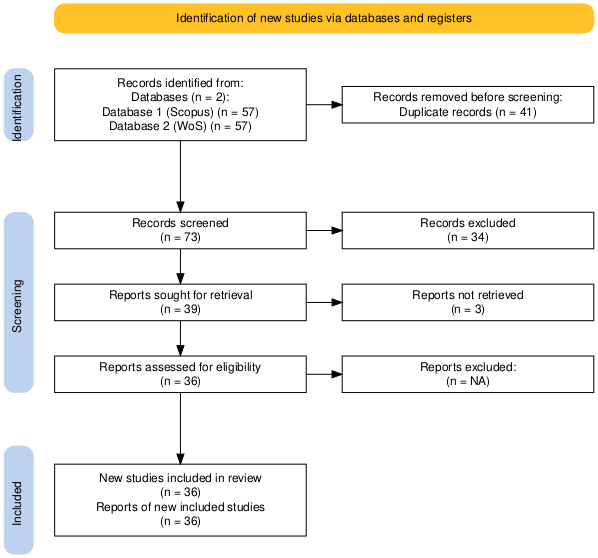
\includegraphics[width=0.8\textwidth]{prisma.png}
    \caption{Diagrama de flujo PRISMA 2020 para el proceso de selección de estudios.}
    \label{fig:prisma}
\end{figure}

La búsqueda inicial arrojó 57 registros en Scopus y 57 en Web of Science, totalizando 114 registros. Tras eliminar 41 duplicados, se obtuvieron 73 registros para filtrar por título y abstract, de los cuales se excluyeron 34 por no cumplir los criterios de relevancia temática. De los 39 artículos buscados seleccionados, 3 no pudieron ser obtenidos por restricciones de acceso. El corpus final de análisis quedó conformado por \textbf{36 artículos}.

\subsection{Criterios de Inclusión y Exclusión}

Los criterios de inclusión fueron, estudios que apliquen al menos una técnica de análisis geoespacial o teledetección, que el contexto de aplicación sea el conflicto Rusia-Ucrania o sus impactos directos, publicados en inglés entre 2022 y 2026 y  disponibles en texto completo. Se excluyeron artículos de opinión, editoriales, comentarios sin datos empíricos, y aquellos que mencionaran técnicas geoespaciales únicamente de forma tangencial.

\clearpage

\subsection{Análisis Bibliométrico}

El análisis bibliométrico se realizó con la librería \texttt{pybibx} de Python sobre los archivos exportados en formato BibTeX desde ambas bases de datos. Se generaron indicadores de producción científica por año, distribución por país, revistas más productivas, autores más citados y mapas de co-ocurrencia de palabras clave.

\subsection{Uso de Inteligencia Artificial en el Proceso de Revisión}

Se utilizaron  herramientas de IA como apoyo en etapas específicas de la revisión. \textbf{Claude Sonnet 4.6} (Anthropic) fue empleado para adaptar los scripts de \texttt{pybibx} al corpus específico y para mejorar la coherencia y redacción . \textbf{NotebookLM} (Google) se utilizó para extraer informacion relevante de los artículos seleccionados, cada respuesta fue contrastada con el texto original antes de incorporarla al análisis para evitar alucinaciones de la ia. La librería \textbf{pybibx} permitió el procesamiento automatizado de metadatos, la generación de gráficos  de indicadores bibliométricos, con selección manual de los resultados más pertinentes.

Todas las decisiones metodológicas como selección de artículos, definición de criterios y redacción final  fueron tomadas por el autor. La tabla detallada de uso de IA por etapa se encuentra en el Material Suplementario (Tabla~S1).

\subsection{Herramientas Computacionales}

Las herramientas utilizadas en la revisión fueron \textbf{Google Colaboratory} como entorno de ejecución principal, donde se corrieron los scripts de \textbf{pybibx} (Python) para el procesamiento y visualización de metadatos bibliométricos, y desde donde se filtraron y revisaron abstracts y otros datos de los artículos.

\clearpage

% ══════════════════════════════════════════════════════════════════════════════
\section{Resultados}
% ══════════════════════════════════════════════════════════════════════════════

\subsection{Caracterización Bibliométrica del Corpus}

La producción científica sobre el conflicto mostró un crecimiento sostenido, con el pico de publicaciones concentrado en 2025, lo que refleja el tiempo necesario para procesar y publicar datos de todo el inicio de la guerra (Figura~\ref{fig:dpy}).

\begin{figure}[H]
    \centering
    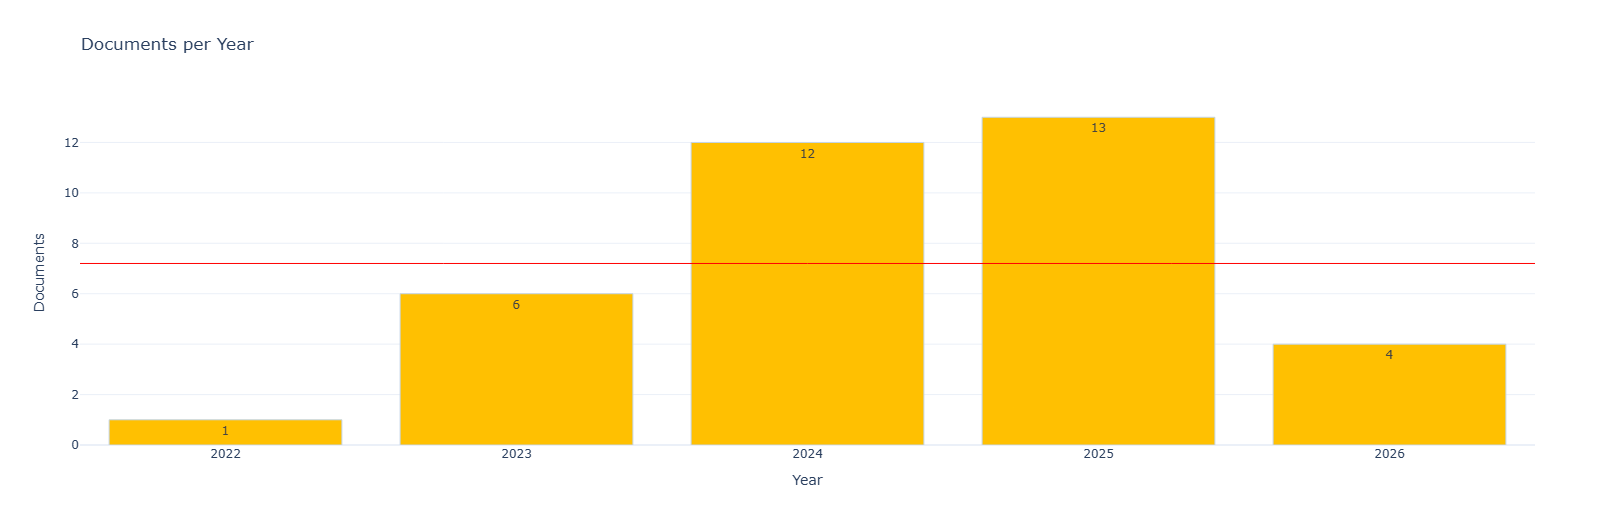
\includegraphics[width=\textwidth, height=5cm, keepaspectratio]{Capturas/dpy.png}
    \caption{Documentos publicados por año sobre análisis geoespacial en el conflicto ruso-ucraniano (2022--2026).}
    \label{fig:dpy}
\end{figure}

En cuanto a la distribución geográfica, China concentra la mayor cantidad de afiliaciones del corpus, seguida de Ucrania, cuyos investigadores colaboran frecuentemente desde el exterior debido al conflicto, y Alemania y Estados Unidos en tercer y cuarto lugar.  (Figura~\ref{fig:cpd}).

\begin{figure}[H]
    \centering
    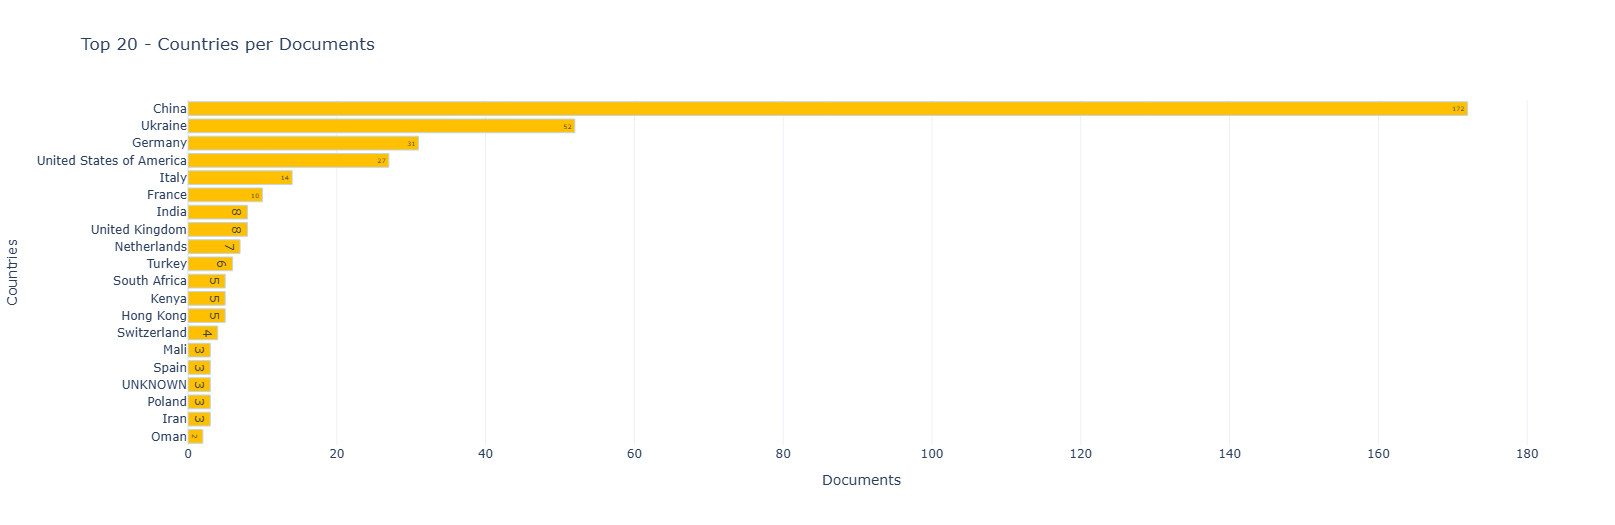
\includegraphics[width=\textwidth, height=5.5cm, keepaspectratio]{Capturas/cpd.png}
    \caption{Países con mayor producción científica sobre análisis geoespacial del conflicto ruso-ucraniano.}
    \label{fig:cpd}
\end{figure}

El análisis de palabras clave (Figura~\ref{fig:wordcloud}) revela que los términos dominantes son \textit{remote, satellite, sensing}, \textit{Ukraine}, \textit{war damage}, \textit{conflict} y \textit{cropland}, confirmando la orientación del corpus hacia la teledetección aplicada a impactos territoriales. La red de co-ocurrencia (Figura~\ref{fig:network}) muestra  clústeres temáticos como daño urbano y evaluación SAR, agricultura y cambio de uso del suelo, calidad ambiental y emisiones y desplazamiento poblacional y luz nocturna.

\begin{figure}[H]
    \centering
    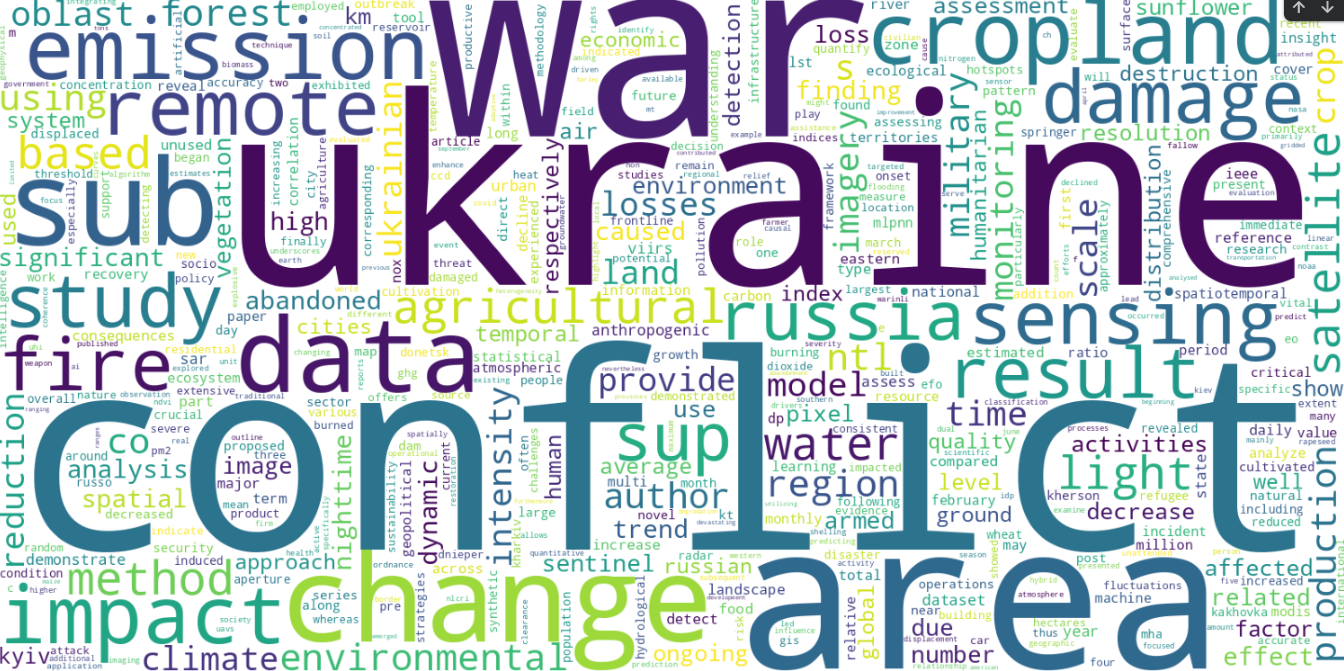
\includegraphics[width=0.85\textwidth]{Capturas/word_cloud.png}
    \caption{Nube de palabras clave más frecuentes en el corpus analizado.}
    \label{fig:wordcloud}
\end{figure}

\begin{figure}[H]
    \centering
    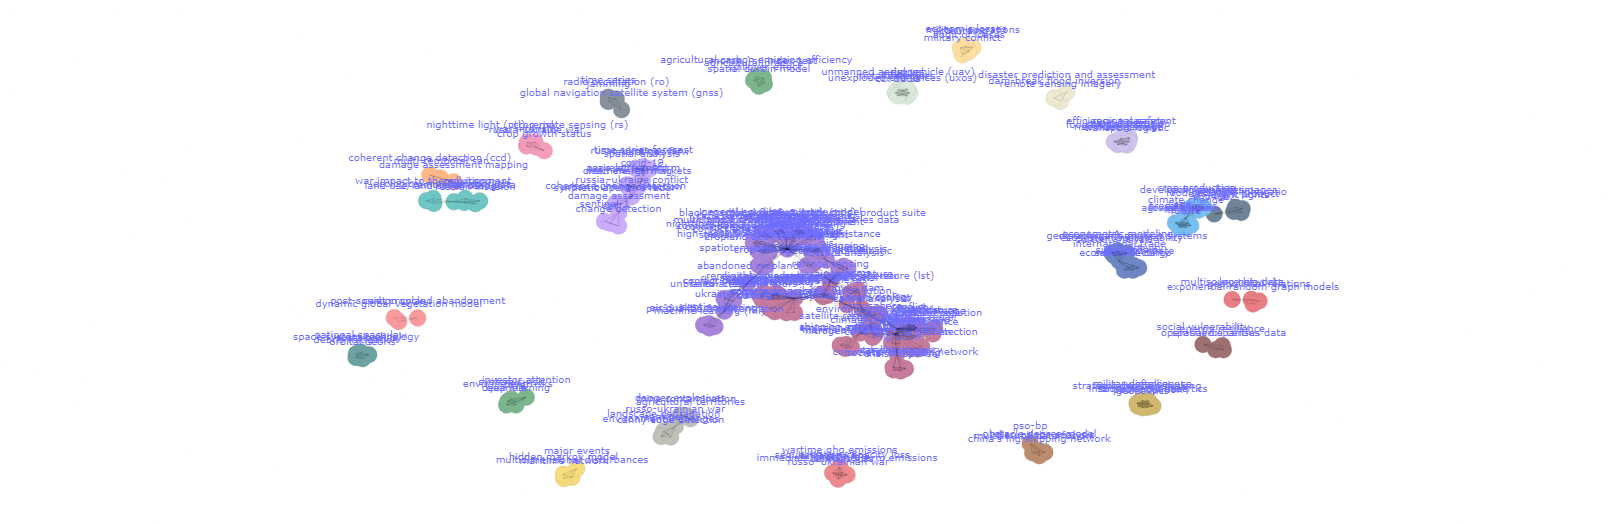
\includegraphics[width=\textwidth, height=7cm, keepaspectratio]{Capturas/network_adj.png}
    \caption{Red de co-ocurrencia de palabras clave (mínimo 2 co-ocurrencias).}
    \label{fig:network}
\end{figure}

El mapa de colaboración internacional (Figura~\ref{fig:map}) muestra que los estudios sobre el conflicto ruso-ucraniano son predominantemente producto de colaboraciones entre instituciones de Europa occidental, Norteamérica y algunas regiones de asi, con participación de investigadores ucranianos en el extranjero.

\begin{figure}[H]
    \centering
    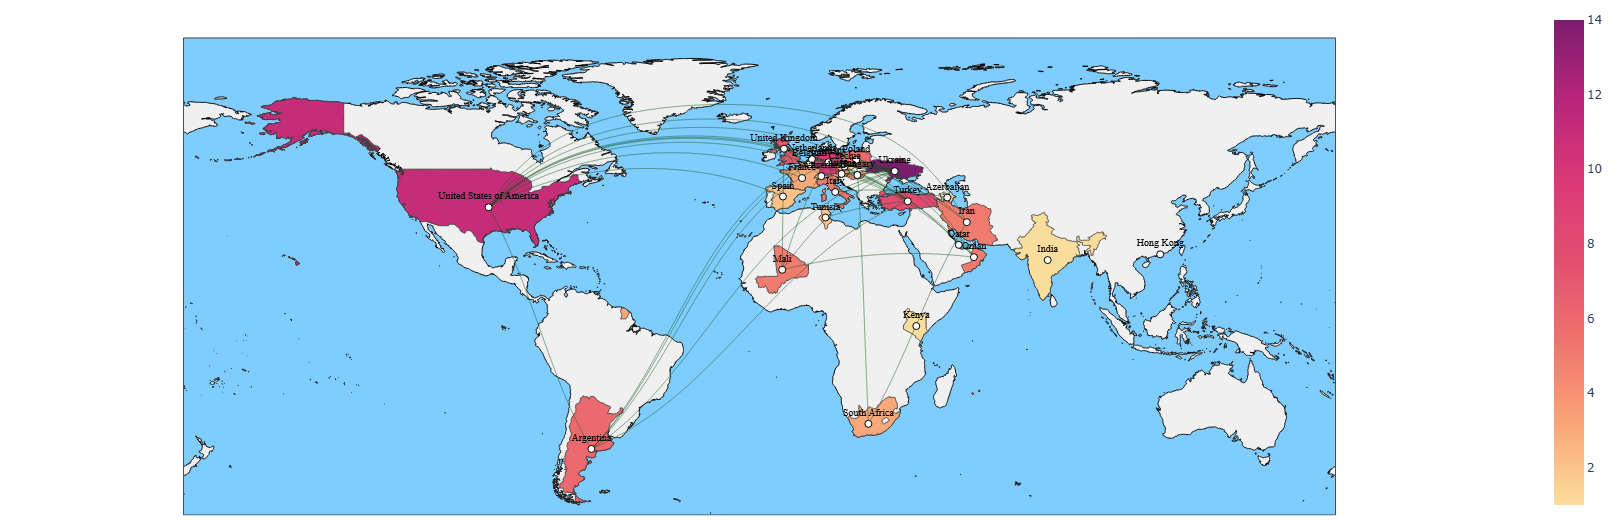
\includegraphics[width=\textwidth, height=6cm, keepaspectratio]{Capturas/network_adj_map.png}
    \caption{Mapa de colaboración científica internacional entre países del corpus.}
    \label{fig:map}
\end{figure}

Los indicadores complementarios como citas acumuladas, autores más productivos, fuentes y bigramas se presentan en el Material Suplementario (Figuras S6--S11).

\subsection{Métodos de Análisis Geoespacial Identificados}

El corpus analizado revela una amplia variedad de metodologías geoespaciales aplicadas al estudio del conflicto ruso-ucraniano. A continuación se sistematizan los principales métodos identificados en el Cuadro~\ref{tab:metodos}.

% ── Tabla de métodos ──────────────────────────────────────────────────────────
\begin{table}[H]
\centering
\singlespacing
\caption{Principales métodos de análisis geoespacial identificados en la literatura.}
\label{tab:metodos}
\footnotesize
\renewcommand{\arraystretch}{1.08}
\begin{tabularx}{\textwidth}{>{\bfseries\color{primary}\raggedright\arraybackslash}p{3.6cm} >{\raggedright\arraybackslash}p{3.0cm} >{\raggedright\arraybackslash}X}
\rowcolor{tableheader}
{\color{white}\bfseries Método} & {\color{white}\bfseries Datos} & {\color{white}\bfseries Principal hallazgo} \\
\midrule
Det. Cambios Coherentes (CCD) SAR & Sentinel-1, GHS-BUILT-S & 264 km² de daño; 67\% a $<$10 km del frente \\

\rowcolor{tablerow}
Machine Learning (RF, XGBoost, DNN) & Sentinel-1/2, VIIRS, ACLED & Pérdida del 82.6\% del área de siembra de girasol \\

Análisis luz nocturna (NTL) umbral dual & VIIRS Black Marble VNP46A2 & Caída del 84\% en intensidad lumínica nacional \\

\rowcolor{tablerow}
Muestreo estratificado + regresión panel & Planet (5m), Sentinel-1/2, ACLED & Fuerte asociación frente-abandono agrícola \\

Análisis espectral (NDVI, NDWI) & Sentinel-2, Landsat-8 & Declive severo de vegetación en el este de Ucrania \\

\rowcolor{tablerow}
Escenarios contrafactuales con ML & Landsat-7/8, Sentinel-1/2, ERA5 & 47.77\% de cuadrículas con reducción productiva en 2022 \\

Inversión satelital validada GEOS-Chem & TROPOMI (NO2), EDGAR, GCP & Caídas en emisiones de NOx y CO2 por cese industrial \\

\rowcolor{tablerow}
Det. Cambios Doble Período (DCD) & MODIS NDVI, Landsat 8-9 & 462{,}000 hectareas abandonadas en el este \\

Visión por computadora + Modelos GAM & Maxar WorldView, WorldPop & Estimación del desplazamiento civil de este a oeste \\

\rowcolor{tablerow}
Análisis puntos calientes Getis-Ord Gi* & MODIS LST, Sentinel-5P, FIRMS & Anomalías térmicas e islas de calor urbano \\
\bottomrule
\end{tabularx}
\end{table}

\clearpage
\subsection{Tecnologías Satelitales más Utilizadas}

El análisis de los 36 artículos evidencia una clara hegemonía de programas de la Agencia Espacial Europea (ESA). Los satélites de la familia Sentinel concentran la mayoría de las aplicaciones, complementados por los sensores de la NASA para monitoreo térmico y nocturno.

\textbf{Sentinel-1 (SAR):} Es el sensor más versátil dado que su tecnología de microondas penetra nubes, lluvia y humo de batalla, permitiendo observación continua independientemente de las condiciones atmosféricas. Se utiliza principalmente para evaluación de daños urbanos mediante Detección de Cambios Coherentes (CCD) y mapeo de abandono de cultivos (Scher \& Van Den Hoek, 2025; Huang et al., 2023).

\textbf{Sentinel-2 (óptico multiespectral):} Con resoluciones de 10 a 20 metros, es la fuente principal para cálculo de índices de vegetación (NDVI, NDWI), monitoreo de inundaciones y detección de áreas quemadas (Hsu, 2024; Lu et al., 2024; Noorali et al., 2025).

\textbf{VIIRS / NASA Black Marble:} Los productos de luz nocturna derivados del sensor VIIRS constituyen la herramienta por excelencia para rastrear cortes energéticos, desplazamiento de población y deterioro de infraestructura a escala nacional y local (Wang et al., 2024; Lin et al., 2024; Guo et al., 2025; Xiao et al., 2024).

\textbf{MODIS:} Ampliamente utilizado para detección de focos de calor (FIRMS), series temporales de vegetación y temperatura superficial terrestre (LST) (Kganyago et al., 2025; Serhii et al., 2022; Gupta \& Shukla, 2024).

\textbf{Satélites comerciales VHR (Planet, Maxar):} Utilizados para validación a nivel de calle, conteo de vehículos en rutas de evacuación e inspección de daños individuales en edificaciones (Rufener et al., 2024; Zatserkovnyi et al., 2025).

\subsection{Cobertura Geográfica}

Los estudios se concentran predominantemente en las regiones orientales y meridionales de Ucrania, correspondientes a las zonas de mayor intensidad de combate y ocupación territorial. Las regiones más estudiadas son los oblasts de \textbf{Donetsk y Luhansk} (producción agrícola y destrucción urbana) (Wagner et al., 2025; Qiu et al., 2026), \textbf{Jersón y Zaporiyia} (abandono de tierras e impacto de la destrucción de la presa de Kajovka) (Mhanna et al., 2026; Lu et al., 2024), \textbf{Járkov} (infraestructura urbana e islas de calor) (Gupta \& Shukla, 2024; Zhang et al., 2023) y \textbf{Kiev y su oblast} (fase inicial de la guerra y calidad del aire) (Mao et al., 2025; Zhang et al., 2023). \textbf{Mariúpol} emerge como el caso de estudio individual más citado, siendo utilizado para calibrar algoritmos de detección de daños urbanos con SAR (Huang et al., 2023; Scher \& Van Den Hoek, 2025).

\subsection{Tipos de Impacto más Documentados}

\begin{tcolorbox}[
    colback=lightbg,
    colframe=primary,
    arc=4pt,
    boxrule=0.6pt,
    title={\bfseries\color{white} Jerarquía de documentación científica},
    coltitle=white,
    fonttitle=\small\bfseries,
    attach boxed title to top left={yshift=-2mm, xshift=4mm},
    boxed title style={colback=primary, arc=2pt}
]
\begin{enumerate}
    \item \textbf{\color{primary}Impactos ambientales} — Muy alta documentación: incendios y pérdida forestal (Cazzolla Gatti et al., 2025; Kganyago et al., 2025), contaminación atmosférica (Roshan et al., 2024; Mao et al., 2025) y desastres hídricos como la destrucción de la presa de Kajovka (Mhanna et al., 2026; Gleick et al., 2023).
    \item \textbf{\color{primary}Impactos agrícolas} — Muy alta documentación: abandono de tierras (Wagner et al., 2025; Zhang, Y., et al., 2025), caída de rendimientos en girasol, trigo y maíz (Qiu et al., 2026; Li et al., 2026).
    \item \textbf{\color{primary}Impactos urbanos e infraestructurales} — Alta documentación: daños en edificaciones (Scher \& Van Den Hoek, 2025; Huang et al., 2023), apagones masivos con caída $>$80\% en luz nocturna (Wang et al., 2024; Lin et al., 2024).
    \item \textbf{\color{primary}Impactos humanitarios} — Documentación indirecta: flujo de refugiados estimado mediante proxies satelitales (Guo et al., 2025; Rufener et al., 2024).
    \item \textbf{\color{primary}Impactos militares} — Documentación contextual: mapeo de líneas de frente como variable causal (Tomchenko et al., 2023; Serhii et al., 2022).
\end{enumerate}
\end{tcolorbox}

% ══════════════════════════════════════════════════════════════════════════════
\section{Discusión}
% ══════════════════════════════════════════════════════════════════════════════

\begin{multicols}{2}

\subsection{Comparación de Enfoques y Estado del Arte}

Ninguno de los estudios revisados utiliza un método único, el patrón que aparece de forma consistente es la \textbf{fusión multisensor}. Los trabajos que combinan SAR (Sentinel-1), óptico (Sentinel-2) y luz nocturna (VIIRS) logran resultados más sólidos que los que dependen de una sola plataforma, porque cada sensor cubre los puntos ciegos de los demás (Scher \& Van Den Hoek, 2025; Hsu, 2024; Wang et al., 2024). En conflictos anteriores como Siria o Yemen el enfoque mono-sensor era habitual; el corpus ucraniano muestra que eso ya no es suficiente.

En Machine Learning, el \textbf{modelado contrafactual} —entrenado con datos 2019--2021 para simular el escenario sin guerra— resulta más preciso que la comparación directa pre/post para aislar el efecto real del conflicto. La diferencia está en el control estadístico de la variabilidad climática y las tendencias de uso del suelo preexistentes (Li et al., 2026; Qiu et al., 2026; Zhang, C., et al., 2024). Los modelos de clasificación supervisada (Random Forest, XGBoost) son más ágiles de implementar, pero no consiguen separar con igual precisión el daño bélico de los cambios naturales del terreno.

Los trabajos que cruzan datos satelitales con \textbf{ACLED y FIRMS} son los que establecen relaciones causales, no solo correlaciones, entre la distancia al frente y la magnitud del daño (Tomchenko et al., 2023; Kganyago et al., 2025). Sin ese cruce, la evidencia satelital queda sin anclaje en los hechos del conflicto. \textbf{Google Earth Engine}, a su vez, no es simplemente una opción cómoda: analizar más de 17,000 asentamientos en todo el territorio ucraniano sería inviable en infraestructura local, independientemente del algoritmo utilizado (Zatserkovnyi et al., 2025; Scher \& Van Den Hoek, 2025).

Comparado con los análisis de conflictos previos, el corpus presenta dos saltos concretos. El primero el uso de luz nocturna con resolución diaria,en lugar de promedios mensuales, que permitieron capturar la ofensiva sobre Kiev de menos de 40 días y reconstruir su cronología completa (Wang et al., 2024; Xiao et al., 2024). El segundo, visión por computadora sobre imágenes de 30 cm para contar vehículos en rutas de evacuación y estimar flujos de refugiados sin datos censales, una aplicación sin antecedentes a esta escala en un conflicto activo (Rufener et al., 2024).

\subsection{Limitaciones Metodológicas}

Los 36 estudios comparten una limitación que ninguno logra resolver completamente, pues sin acceso al terreno, no hay validación en el sitio. Los campos minados y la actividad de combate hacen inviable la recolección directa de datos en las zonas más afectadas (Scher \& Van Den Hoek, 2025; Wagner et al., 2025). En el plano técnico, los \textbf{sensores ópticos} acusan la nubosidad persistente, el humo de bombardeos y la nieve estacional del este ucraniano (Hsu, 2024; Lu et al., 2024); los \textbf{sensores SAR}, por su lado, no distinguen cultivos de baja estatura y pierden resolución al intentar evaluar daños a nivel de edificio individual (Huang et al., 2023). Un punto débil frecuente adicional es interpretar la caída de luz nocturna directamente como desplazamiento de personas, sin considerar toques de queda o cortes eléctricos planificados como posibles explicaciones alternativas (Guo et al., 2025; Lin et al., 2024).

La \textbf{reproducibilidad} es heterogénea. Algunos grupos comparten código en GitHub (Rufener et al., 2024; Zhang, S., et al., 2025) y datos procesados en Zenodo, otros solo los entregan bajo solicitud directa al autor. Los datos base —Sentinel (ESA), VIIRS, MODIS, Landsat (NASA/USGS)— son de acceso abierto y procesables en Google Earth Engine, lo que asegura la reproducibilidad del enfoque general. La excepción son las imágenes comerciales de muy alta resolución (Maxar, Planet), cuya confidencialidad impide redistribuirlas (Rufener et al., 2024).

\subsection{Vacíos en la Literatura}

Entre los 36 artículos, \textbf{ninguno parte del evento de combate como unidad de análisis}. Los estudios detectan daño desde el satélite y luego buscan correlación con el conflicto como variable explicativa, pero no al revés, no se agrupa dónde ocurren los ataques, ni se construye con eso un índice de riesgo territorial para la población civil. La diferencia no es menor: un análisis desde el terreno permitiría cruzar la distribución espacial de los combates con el daño documentado satelitalmente, cerrando el ciclo explicativo que el corpus actual deja abierto.

\subsection{Líneas de Investigación Futura}

Los propios autores apuntan en varias direcciones. El paso técnico más señalado es integrar \textbf{Deep Learning} para automatizar la detección de daños con mayor precisión (Zatserkovnyi et al., 2025; Qiu et al., 2026). En paralelo, una \textbf{fusión multisensor} más sistemática reduciría las brechas causadas por nubosidad y limitaciones de resolución (Scher \& Van Den Hoek, 2025; Li et al., 2026). Para el seguimiento de población desplazada, los datos de dispositivos móviles y redes sociales ofrecen una alternativa más directa que los proxies lumínicos actuales (Rufener et al., 2024). Finalmente, los marcos desarrollados en Ucrania —CCD, modelado contrafactual, fusión multisensor— son transferibles a otros contextos de conflicto como Sudán, Gaza o Myanmar (Scher \& Van Den Hoek, 2025; Wagner et al., 2025).

Como extensión concreta de este trabajo, se propone aplicar \textbf{K-Means} sobre los registros georreferenciados de ACLED para agrupar los eventos de bombardeo e identificar las zonas del territorio ucraniano con mayor concentración de ataques y combates.

\end{multicols}

\vspace

% ══════════════════════════════════════════════════════════════════════════════
\section{Conclusiones}
% ══════════════════════════════════════════════════════════════════════════════

\begin{multicols}{2}

Los artículos analizados publicados entre 2022 y 2026, permiten responder directamente la pregunta planteada. Los métodos más frecuentes son la detección de cambios coherentes con SAR (Sentinel-1), el modelado contrafactual con Machine Learning y el análisis de luz nocturna con VIIRS, aplicados principalmente en las regiones orientales y meridionales de Ucrania para documentar impactos agrícolas, urbanos y ambientales.

En todos los estudios el satélite operó como sustituto del trabajo de campo. Los hallazgos son coherentes entre sí, ~2.4 millones de hectáreas agrícolas abandonadas, 264 km² de daño urbano distribuido en más de 2,288 asentamientos, caída del 84\% en la intensidad lumínica nacional y más de 6.33 millones de desplazados estimados mediante proxies satelitales.

El punto ciego común es que ninguno de los 36 papers agrupa los eventos de combate en tierra, todos detectan daño desde arriba, pero no existe un índice que caracterice la intensidad del conflicto desde el origen de los ataques. La validación sigue siendo el problema sin resolver, acceder a las zonas de combate para verificar los resultados satelitales es, por ahora, inviable.

Los marcos que este corpus construyó —CCD, modelado contrafactual, fusión multisensor son trasladables a otros conflictos activos, lo que posiciona el caso ucraniano como referencia metodológica para el análisis geoespacial de crisis. Como paso siguiente en el proyecto semestral, se propone aplicar K-Means sobre los datos de ACLED para agrupar los eventos de bombardeo y mapear la intensidad del conflicto desde el terreno, cruzando esos resultados con el daño documentado satelitalmente.

\end{multicols}

\clearpage

\FloatBarrier

% ══════════════════════════════════════════════════════════════════════════════
% DECLARACIÓN DE USO DE IA
% ══════════════════════════════════════════════════════════════════════════════
\section*{Declaración de uso de inteligencia artificial}
\addcontentsline{toc}{section}{Declaración de uso de inteligencia artificial}

Durante la elaboración de este trabajo se utilizó el modelo de lenguaje \textbf{Claude Sonnet 4.6} (Anthropic, 2026), accedido a través de la aplicación de escritorio Cowork, como herramienta de apoyo de estructuración y redacción del manuscrito en Latex y revisión de coherencia, verificación del formato de citas y generación de la presentación interactiva en Streamlit. Todas las decisiones metodológicas, la selección y análisis de los artículos del corpus, la interpretación de los resultados y las conclusiones son responsabilidad del autor. El uso de IA se limita a asistencia textual y técnica, no en el diseño ni en el juicio investigativo.

\FloatBarrier

% ══════════════════════════════════════════════════════════════════════════════
% MATERIAL SUPLEMENTARIO
% ══════════════════════════════════════════════════════════════════════════════

\section*{Material Suplementario}
\addcontentsline{toc}{section}{Material Suplementario}

Los siguientes elementos complementan el análisis bibliométrico presentado en el cuerpo principal. No se incluyen en el conteo de figuras del manuscrito.

\subsection*{Tabla S1. Uso de inteligencia artificial por etapa}

\begin{table}[H]
\centering
\footnotesize
\renewcommand{\arraystretch}{1.15}
\begin{tabularx}{\textwidth}{>{\bfseries\raggedright\arraybackslash}p{2.8cm} >{\raggedright\arraybackslash}p{2.4cm} >{\raggedright\arraybackslash}X >{\raggedright\arraybackslash}p{3.2cm}}
\rowcolor{tableheader}
{\color{white}\bfseries Etapa} & {\color{white}\bfseries Herramienta} & {\color{white}\bfseries Uso específico} & {\color{white}\bfseries Verificación humana} \\
\midrule
Formulación del problema & Claude Sonnet 4.6 & Generación de términos clave y estructuración de operadores booleanos & Las cadenas se ejecutaron manualmente en Scopus y WoS; la selección de artículos fue propia \\
\rowcolor{tablerow}
Búsqueda bibliográfica & NotebookLM & Extracción de información relevante de los artículos seleccionados & Cada dato extraído fue verificado y contrastado con el paper original antes de usarlo \\
Extracción de datos & pybibx (Python) & Generación de tablas, gráficos e indicadores bibliométricos & Se revisaron los outputs y se eligieron los gráficos e indicadores más representativos \\
\rowcolor{tablerow}
Síntesis y redacción & Claude Sonnet 4.6 & Mejora de coherencia y redacción & El texto fue revisado y editado de forma iterativa hasta la versión final \\
\bottomrule
\end{tabularx}
\caption*{\textbf{Tabla S1.} Declaración de uso de inteligencia artificial por etapa del proceso de revisión.}
\end{table}

\subsection*{S2. Cadenas de búsqueda completas por base de datos}

\begin{tcolorbox}[colback=lightbg, colframe=accent, arc=3pt, boxrule=0.6pt,
    left=8pt, right=8pt, top=6pt, bottom=6pt,
    title={\small\bfseries Cadena A — Scopus y WoS (1 de mayo de 2026)},
    coltitle=primary, fonttitle=\small\bfseries]
\small\ttfamily
(``Ukraine war'' OR ``Ukraine conflict'' OR ``Russo-Ukrainian war'' OR ``Russia-Ukraine'')\\
AND\\
(``spatial analysis'' OR ``geospatial'' OR ``GIS'' OR ``remote sensing'' OR\\
``satellite imagery'' OR ``spatial pattern*'' OR ``geographic information'')
\end{tcolorbox}

\begin{tcolorbox}[colback=lightbg, colframe=accent, arc=3pt, boxrule=0.6pt,
    left=8pt, right=8pt, top=6pt, bottom=6pt,
    title={\small\bfseries Cadena B — solo WoS (1 de mayo de 2026)},
    coltitle=primary, fonttitle=\small\bfseries]
\small\ttfamily
``Ukraine war'' OR ``Ukraine conflict'' OR ``Russo-Ukrainian war''\\
AND\\
``Spatial analysis'' OR ``Geospatial'' OR ``GIS'' OR ``Spatial pattern*''
\end{tcolorbox}

\subsection*{S3. Capturas de registros de búsqueda}

\begin{figure}[H]
    \centering
    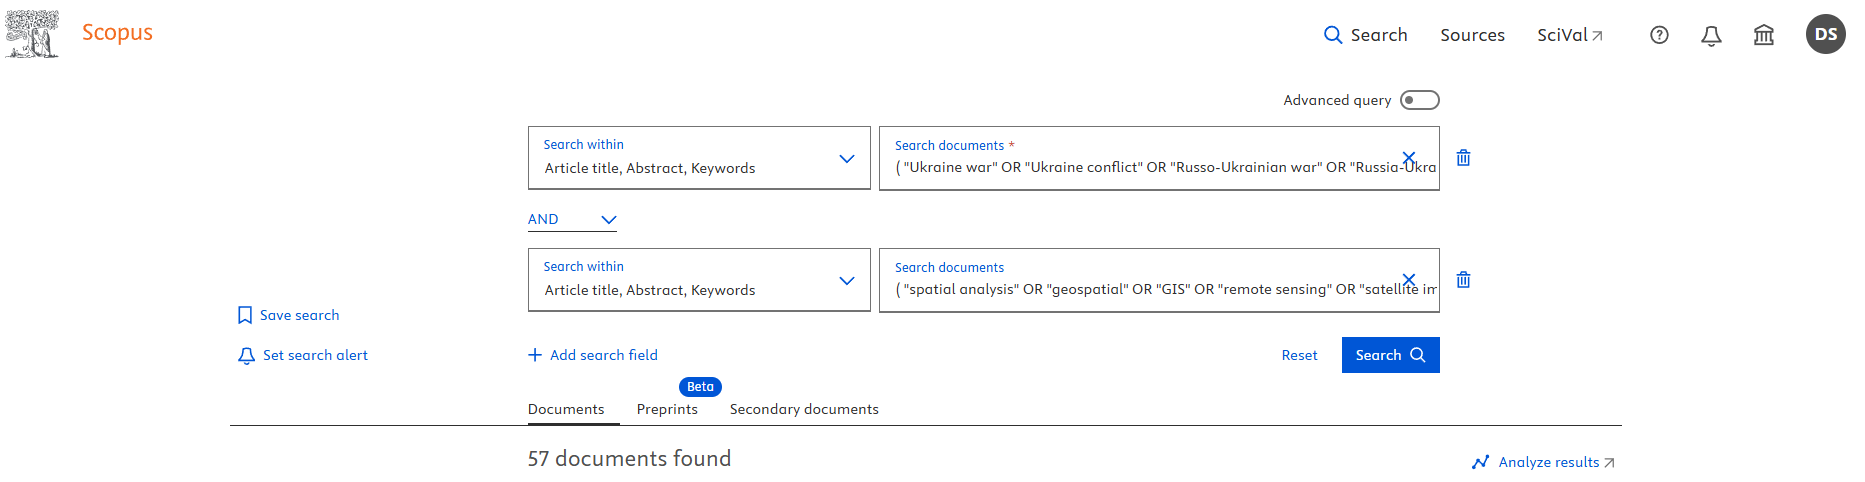
\includegraphics[width=\textwidth, keepaspectratio]{Capturas/busqueda1.png}
    \caption*{\textbf{Figura S3a.} Captura de resultados de búsqueda — Scopus.}
\end{figure}

\begin{figure}[H]
    \centering
    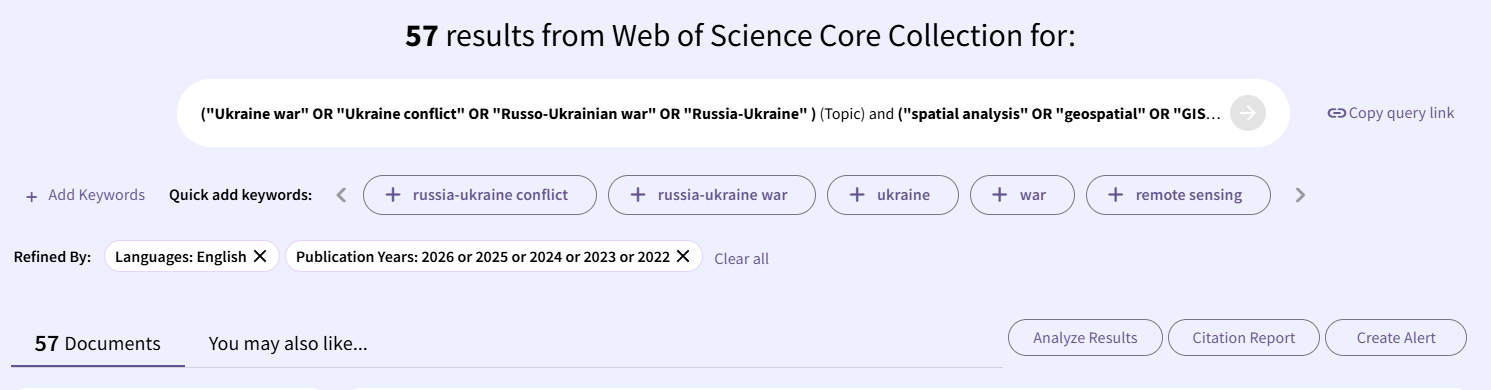
\includegraphics[width=\textwidth, keepaspectratio]{Capturas/busqueda2.png}
    \caption*{\textbf{Figura S3b.} Captura de resultados de búsqueda — Web of Science (Cadena A).}
\end{figure}

\begin{figure}[H]
    \centering
    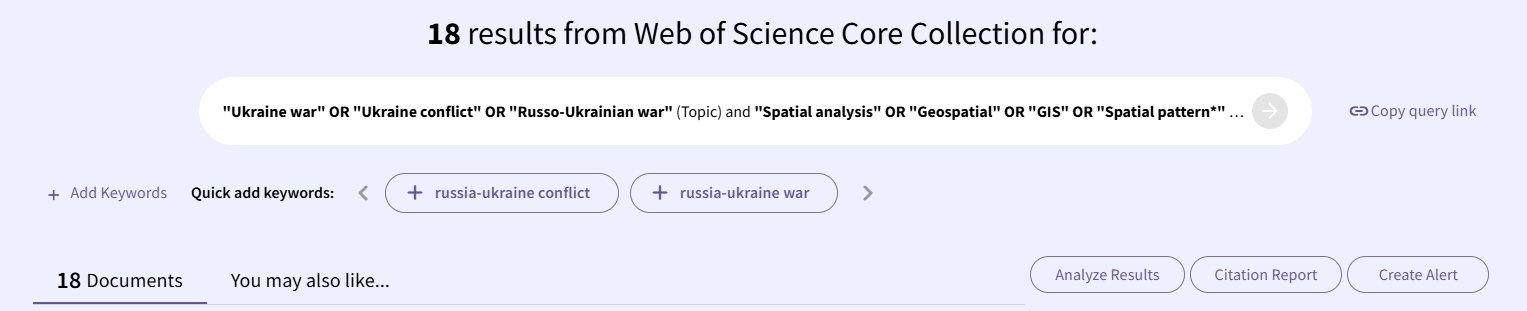
\includegraphics[width=\textwidth, keepaspectratio]{Capturas/busqueda3.png}
    \caption*{\textbf{Figura S3c.} Captura de resultados de búsqueda — Web of Science (Cadena B).}
\end{figure}

\subsection*{S4. Criterios de inclusión y exclusión aplicados}

\begin{table}[H]
\centering
\footnotesize
\renewcommand{\arraystretch}{1.15}
\begin{tabularx}{\textwidth}{>{\bfseries\raggedright\arraybackslash}p{2cm} >{\raggedright\arraybackslash}X}
\rowcolor{tableheader}
{\color{white}\bfseries Tipo} & {\color{white}\bfseries Criterio} \\
\midrule
Inclusión & Aplica al menos una técnica de análisis geoespacial o teledetección \\
\rowcolor{tablerow}
Inclusión & Contexto de aplicación es el conflicto Rusia-Ucrania o sus impactos directos \\
Inclusión & Publicado en inglés entre 2022 y 2026 \\
\rowcolor{tablerow}
Inclusión & Disponible en texto completo \\
Exclusión & Artículos de opinión, editoriales o comentarios sin datos empíricos \\
\rowcolor{tablerow}
Exclusión & Técnicas geoespaciales mencionadas solo de forma tangencial \\
Exclusión & Sin acceso a resumen o texto completo \\
\rowcolor{tablerow}
Exclusión & Estudios duplicados entre bases de datos \\
\bottomrule
\end{tabularx}
\caption*{\textbf{Tabla S4.} Criterios de inclusión y exclusión aplicados en la selección del corpus.}
\end{table}

\subsection*{S5. Código, datos y repositorio}

El código completo utilizado para el procesamiento bibliométrico, generación de gráficos e indicadores con \texttt{pybibx}, así como la tabla con los 36 artículos seleccionados (año, título y abstract), se encuentran disponibles en el siguiente repositorio de Google Colaboratory:

\begin{tcolorbox}[colback=lightbg, colframe=accent, arc=3pt, boxrule=0.6pt,
    left=8pt, right=8pt, top=6pt, bottom=6pt]
\small\ttfamily\raggedright
\url{https://colab.research.google.com/drive/1w7vu7xPYRZaBOxYMVbpfmJ7b1sjR5aP8?usp=sharing}
\end{tcolorbox}

\subsection*{S6. Citas acumuladas por año}

\begin{figure}[H]
    \centering
    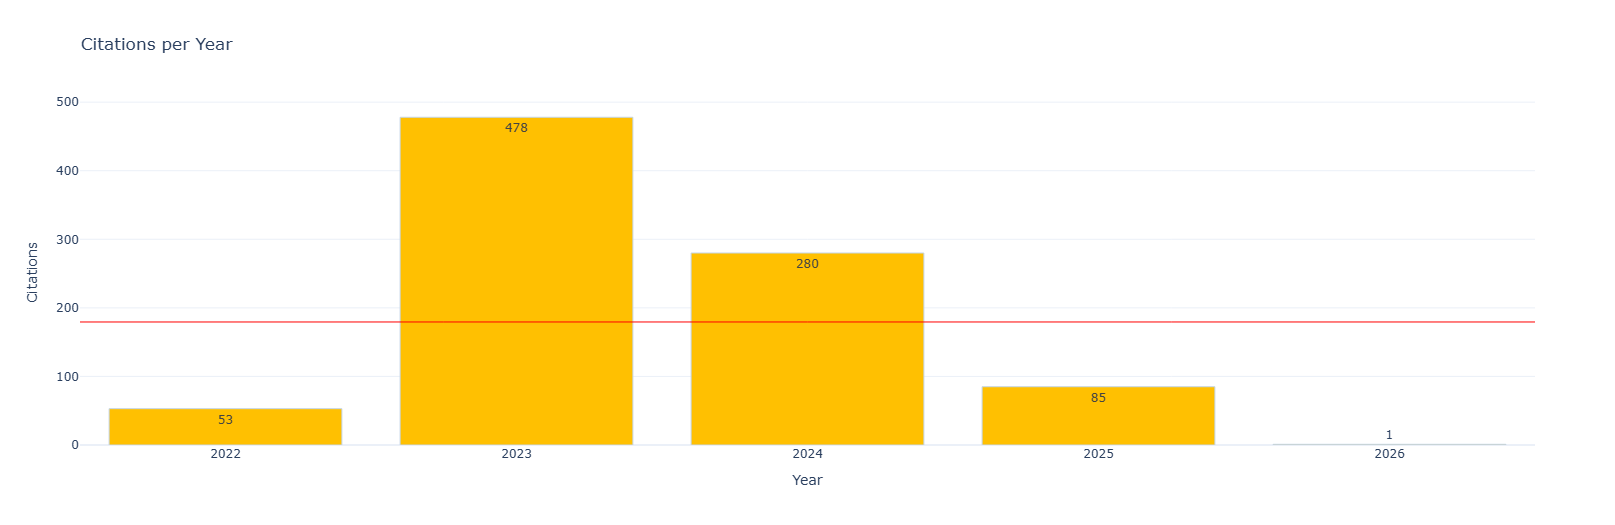
\includegraphics[width=\textwidth, height=5cm, keepaspectratio]{Capturas/cpy.png}
    \caption*{\textbf{Figura S6.} Citas acumuladas por año en el corpus analizado (2022--2026).}
\end{figure}

\subsection*{S7. Autores más productivos}

\begin{figure}[H]
    \centering
    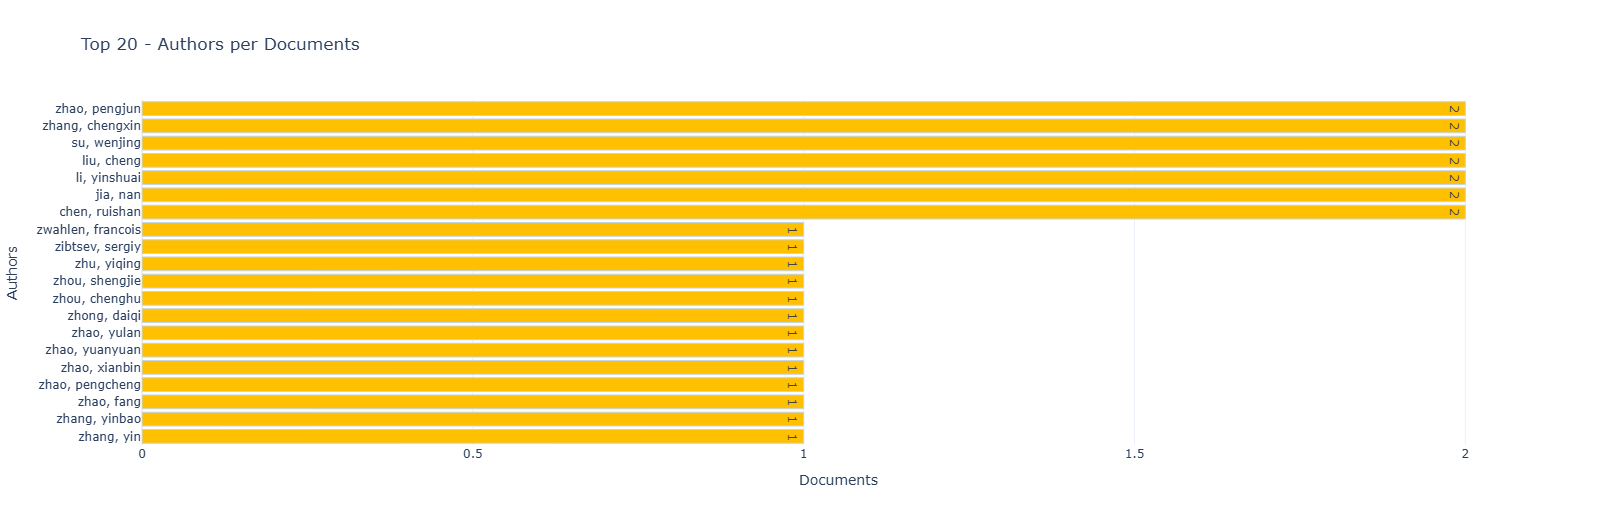
\includegraphics[width=\textwidth, height=5.5cm, keepaspectratio]{Capturas/apd.png}
    \caption*{\textbf{Figura S7.} Autores con mayor número de documentos publicados en el corpus.}
\end{figure}

\subsection*{S8. Fuentes más productivas}

\begin{figure}[H]
    \centering
    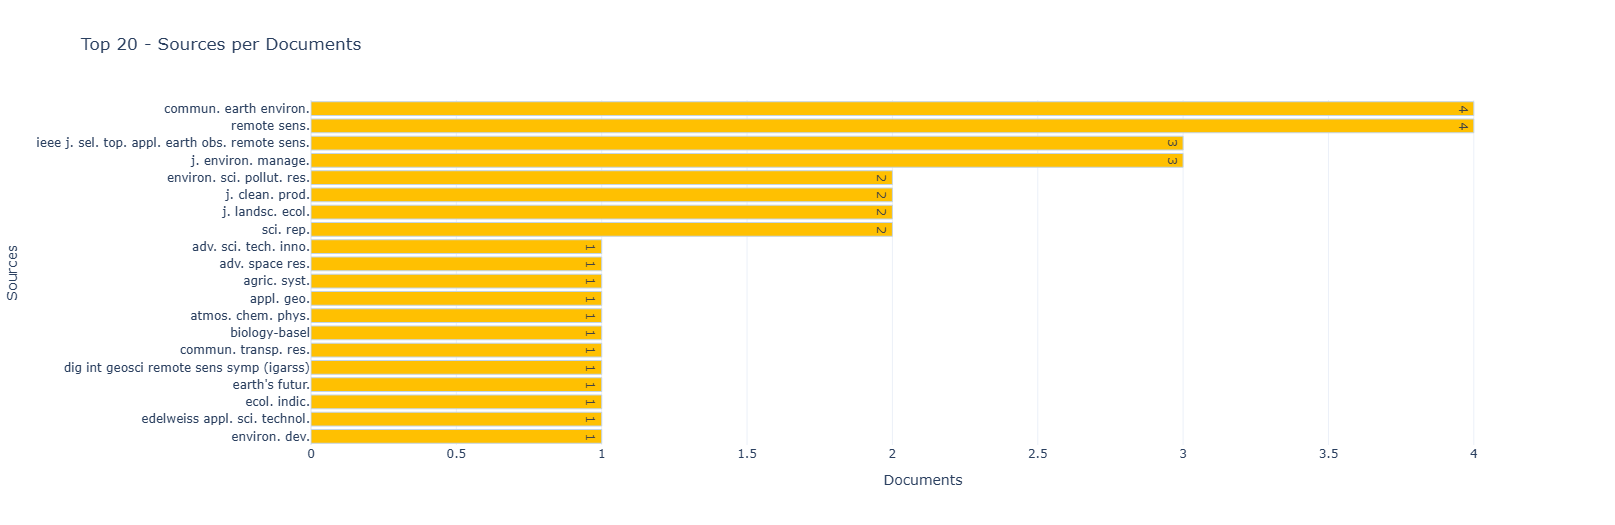
\includegraphics[width=\textwidth, height=5.5cm, keepaspectratio]{Capturas/spd.png}
    \caption*{\textbf{Figura S8.} Revistas con mayor número de documentos publicados.}
\end{figure}

\begin{figure}[H]
    \centering
    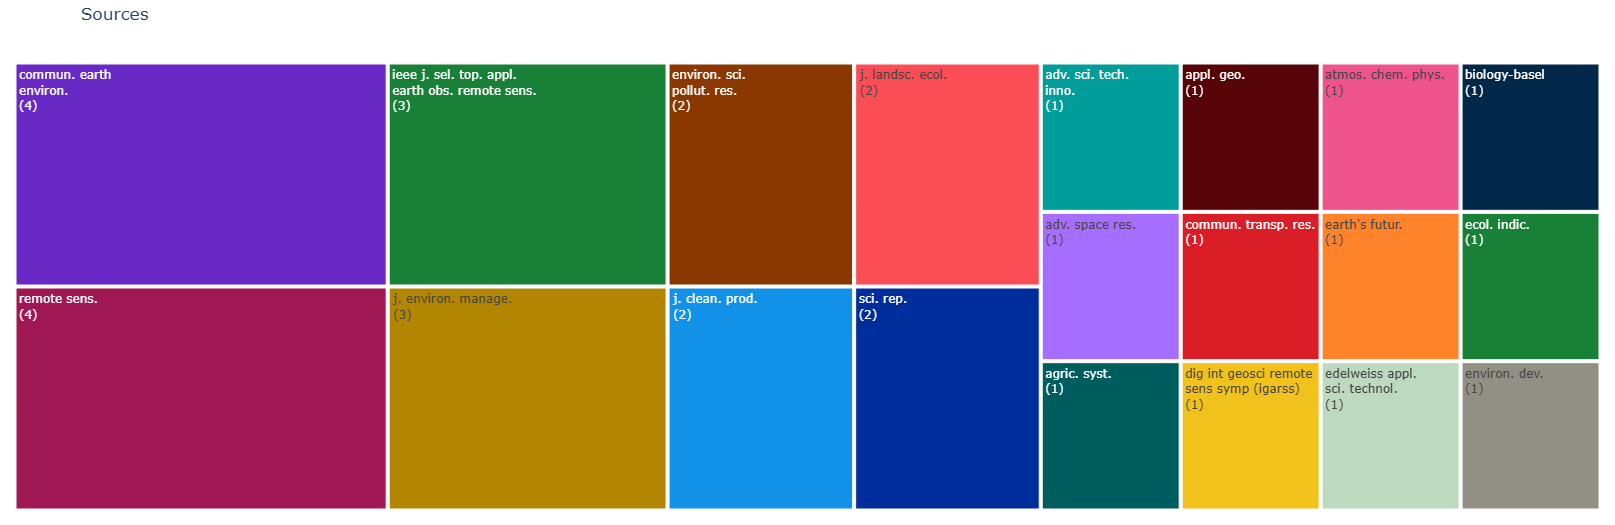
\includegraphics[width=\textwidth, height=6cm, keepaspectratio]{Capturas/tree_map.png}
    \caption*{\textbf{Figura S9.} Distribución proporcional de publicaciones por revista (treemap).}
\end{figure}

\subsection*{S9. Bigramas más frecuentes}

\begin{figure}[H]
    \centering
    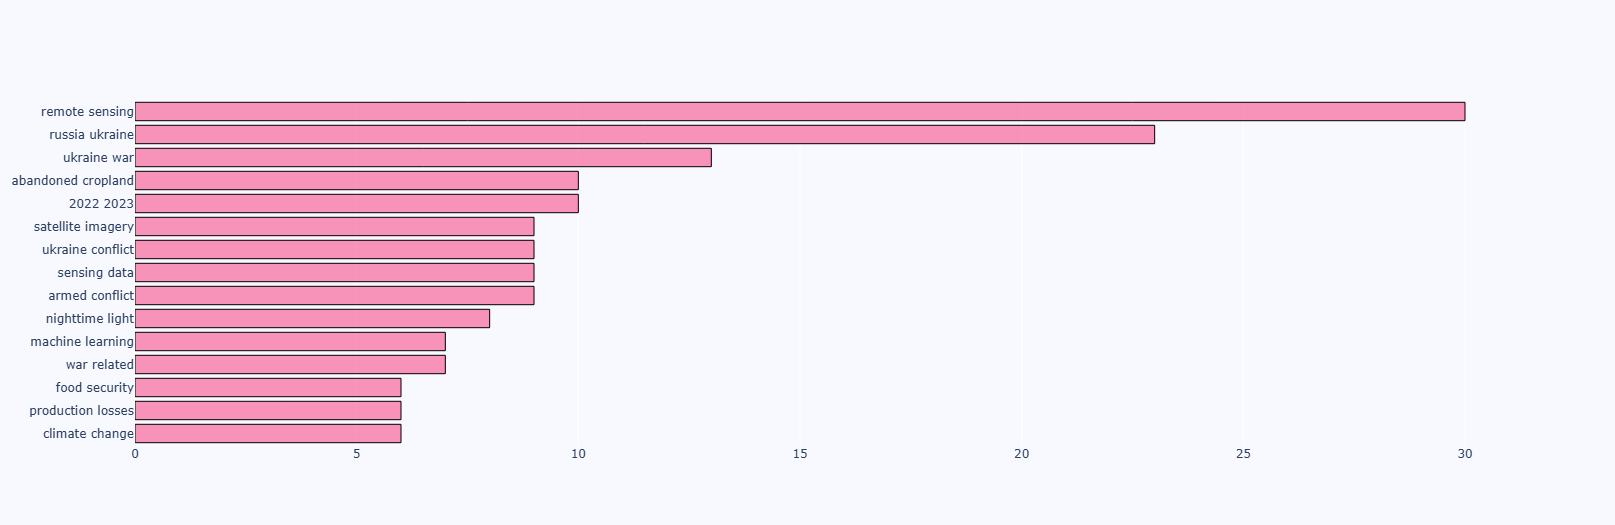
\includegraphics[width=\textwidth, height=5.5cm, keepaspectratio]{Capturas/ngrams.png}
    \caption*{\textbf{Figura S10.} Bigramas más frecuentes en los abstracts del corpus analizado.}
\end{figure}

\subsection*{S10. Flujo de selección bibliográfica (Sankey)}

\begin{figure}[H]
    \centering
    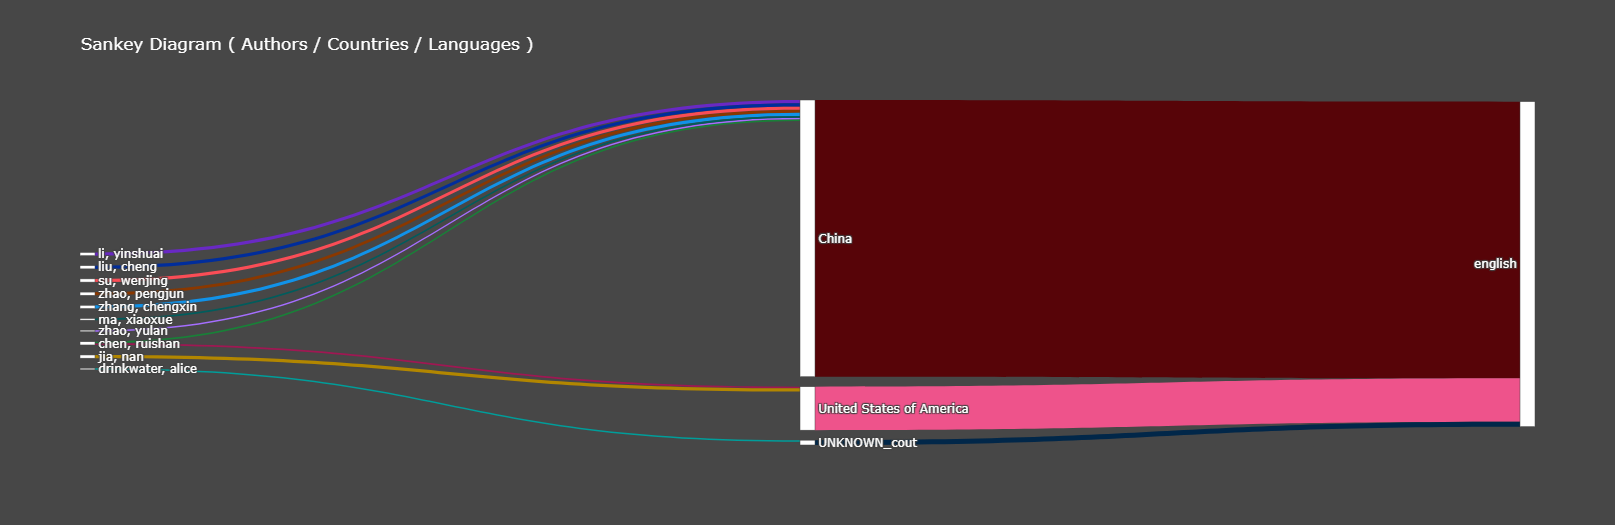
\includegraphics[width=\textwidth, height=6cm, keepaspectratio]{Capturas/sankey.png}
    \caption*{\textbf{Figura S11.} Diagrama Sankey de relaciones entre autores, países e idiomas de publicación.}
\end{figure}

% ══════════════════════════════════════════════════════════════════════════════
% REFERENCIAS
% ══════════════════════════════════════════════════════════════════════════════
\renewcommand{\refname}{Referencias}
\addcontentsline{toc}{section}{Referencias}

\begin{thebibliography}{99}
\small

\bibitem{cazzollagatti2025}
Cazzolla Gatti, R., Cortès Lobos, R. B., Torresani, M., \& Rocchini, D. (2025). An early warning system based on machine learning detects huge forest loss in Ukraine during the war. \textit{Global Ecology and Conservation}, \textit{58}. \url{https://doi.org/10.1016/j.gecco.2025.e03427}

\bibitem{chen2024}
Chen, B., Tu, Y., An, J., Wu, S., Lin, C., \& Gong, P. (2024). Quantification of losses in agriculture production in eastern Ukraine due to the Russia-Ukraine war. \textit{Communications Earth and Environment}, \textit{5}(1). \url{https://doi.org/10.1038/s43247-024-01488-3}

\bibitem{dai2024}
Dai, K., Cheng, C., Kan, S., Li, Y., Liu, K., \& Wu, X. (2024). Impact of Arable Land Abandonment on Crop Production Losses in Ukraine During the Armed Conflict. \textit{Remote Sensing}, \textit{16}(22). \url{https://doi.org/10.3390/rs16224207}

\bibitem{drinkwater2026}
Drinkwater, A. (2026). Field in the frame: Agricultural fires from above. \textit{Communications Earth and Environment}, \textit{7}(1). \url{https://doi.org/10.1038/s43247-026-03496-x}

\bibitem{gleick2023}
Gleick, P., Vyshnevskyi, V., \& Shevchuk, S. (2023). Rivers and Water Systems as Weapons and Casualties of the Russia-Ukraine War. \textit{Earth's Future}, \textit{11}(10). \url{https://doi.org/10.1029/2023EF003910}

\bibitem{guo2025}
Guo, B., Zhang, S., Xie, T., Zhang, W., Wang, Z., Zhang, D., Chen, P., \& Guo, T. (2025). Spatiotemporal dynamics of refugees and displaced persons during the Russia-Ukraine conflict: A nighttime light remote sensing perspective. \textit{Advances in Space Research}, \textit{76}(4), 2053--2071. \url{https://doi.org/10.1016/j.asr.2025.06.009}

\bibitem{gupta2024}
Gupta, P., \& Shukla, D. P. (2024). Implications of Russia–Ukraine war on land surface temperature and air quality: Long-term and short-term analysis. \textit{Environmental Science and Pollution Research}, \textit{31}(34), 46357--46375. \url{https://doi.org/10.1007/s11356-024-32800-5}

\bibitem{hsu2024}
Hsu, F. (2024). Analyzing Vegetation Damage from the Russo-Ukrainian War: A Geographic Information System & Remote Sensing-Based Analysis. \textit{URTC 2024 - 2024 IEEE MIT Undergraduate Research Technology Conference, Proceedings}. \url{https://doi.org/10.1109/URTC65039.2024.10937587}

\bibitem{huang2023}
Huang, Q., Jin, G., Xiong, X., Ye, H., \& Xie, Y. (2023). Monitoring Urban Change in Conflict from the Perspective of Optical and SAR Satellites: The Case of Mariupol, a City in the Conflict between RUS and UKR. \textit{Remote Sensing}, \textit{15}(12). \url{https://doi.org/10.3390/rs15123096}

\bibitem{kganyago2025}
Kganyago, M., Tshigoli, P., \& Shikwambana, L. (2025). Geospatial analysis of the fire incidents and burned areas induced by Russia-Ukraine war in 2022 using MODIS and VIIRS data. \textit{Applied Geomatics}, \textit{17}(3), 519--533. \url{https://doi.org/10.1007/s12518-025-00634-6}

\bibitem{li2026}
Li, Y., Yao, K., Meng, Q., Wang, Y., Xiao, R., Liu, Y., Wu, S., \& Li, Y. (2026). Dynamic patterns and driving factors of productive cropland in Ukraine before and after Russia-Ukraine conflict. \textit{Geography and Sustainability}, \textit{7}(1). \url{https://doi.org/10.1016/j.geosus.2025.100401}

\bibitem{lin2024}
Lin, Y., Gao, C., Yu, J., Li, L., Chen, X., Yang, Y., \& Zhong, D. (2024). Pixel-Level Quantification of Damage and Recovery Caused by the Russia-Ukraine Conflict Based on Nighttime Light Imagery. \textit{IEEE Journal of Selected Topics in Applied Earth Observations and Remote Sensing}, \textit{17}, 14712--14725. \url{https://doi.org/10.1109/JSTARS.2024.3449394}

\bibitem{liu2025}
Liu, Z., Li, J., Chen, H., Wang, L., \& Plaza, A. (2025). Monitoring changes in nighttime lights and anthropogenic CO2 emissions during geopolitical conflicts from a remote sensing perspective. \textit{Humanities and Social Sciences Communications}, \textit{12}(1). \url{https://doi.org/10.1057/s41599-025-05151-w}

\bibitem{lu2024}
Lu, L., Zhu, Y., \& Gu, J. (2024). Detecting the Impacts of Ongoing Russia-Ukraine Conflict on Crop Growth and Human Activity Using Multi-Modal Remote Sensing Time-Series Data. \textit{12th International Conference on Agro-Geoinformatics, Agro-Geoinformatics 2024}. \url{https://doi.org/10.1109/Agro-Geoinformatics262780.2024.10660807}

\bibitem{mao2025}
Mao, Y., Ju, W., Wang, H., Liu, L., Wang, H., Feng, S., Jia, M., \& Jiang, F. (2025). Inversion-based assessment of anthropogenic NOx   emission changes in Ukraine during the 2022-2023 war using TROPOMI   satellite data. \textit{Atmospheric Chemistry and Physics}, \textit{25}(21), 14187-14204. \url{https://doi.org/10.5194/acp-25-14187-2025}

\bibitem{mehrabi2023}
Mehrabi, M., Scaioni, M., \& Previtali, M. (2023). Forecasting Air Quality in Kiev During 2022 Military Conflict Using Sentinel 5P and Optimized Machine Learning. \textit{IEEE Transactions on Geoscience and Remote Sensing}, \textit{61}. \url{https://doi.org/10.1109/TGRS.2023.3292006}

\bibitem{mhanna2026}
Mhanna, S., Scanlon, B. R., Rateb, A., Halloran, L. J. S., Bianco, M., Zwahlen, F., \& Brunner, P. (2026). Hydrological and ecological consequences of the Kakhovka dam collapse. \textit{Environmental Research Letters}, \textit{21}(6). \url{https://doi.org/10.1088/1748-9326/ae4d5f}

\bibitem{noorali2025}
Noorali, H., Zaki, Y., Campana, M., \& Taheri, A. (2025). Hydropolitics of Russian-Ukrainian war: Analyzing water governance conflicts in the Dnieper River basin through remote sensing techniques. \textit{GeoJournal}, \textit{90}(3). \url{https://doi.org/10.1007/s10708-025-11338-0}

\bibitem{qiu2026}
Qiu, J., Hu, Y., Peng, D., Liu, H., Tao, W., Xie, B., Hu, T., Wang, J., Liang, X., Chen, T., \& Xu, J. (2026). Analyzing the disruption of agricultural systems by conflict: A case study of sunflower production in eastern Ukraine. \textit{Agricultural Systems}, \textit{233}. \url{https://doi.org/10.1016/j.agsy.2026.104636}

\bibitem{rodger2023}
Rodger, M., \& Guida, R. (2023). Damage assessment mapping in Mariupol (Ukraine) with multi-temporal   synthetic aperture radar (SAR). \textit{IGARSS 2023 — IEEE International Geoscience and Remote Sensing Symposium}, 7186-7189. \url{https://doi.org/10.1109/IGARSS52108.2023.10281740}

\bibitem{roshan2024}
Roshan, G., Ghanghermeh, A., Sarli, R., \& Grab, S. W. (2024). Environmental impacts of shifts in surface urban heat island, emissions, and nighttime light during the Russia–Ukraine war in Ukrainian cities. \textit{Environmental Science and Pollution Research}, \textit{31}(32), 45246--45263. \url{https://doi.org/10.1007/s11356-024-34050-x}

\bibitem{rufener2024}
Rufener, M., Ofli, F., Fatehkia, M., \& Weber, I. (2024). Estimation of internal displacement in Ukraine from satellite-based car detections. \textit{Scientific Reports}, \textit{14}(1). \url{https://doi.org/10.1038/s41598-024-80035-8}

\bibitem{scher2025}
Scher, C., \& Van Den Hoek, J. (2025). Nationwide conflict damage mapping with interferometric synthetic aperture radar: A study of the 2022 Russia–Ukraine conflict. \textit{Science of Remote Sensing}, \textit{11}. \url{https://doi.org/10.1016/j.srs.2025.100217}

\bibitem{serhii2022}
Serhii, A. S., Vyshnevskyi, V. I., \& Bilous, O. (2022). The Use of Remote Sensing Data for Investigation of Environmental Consequences of Russia-Ukraine War. \textit{Journal of Landscape Ecology(Czech Republic)}, \textit{15}(3), 36--53. \url{https://doi.org/10.2478/jlecol-2022-0017}

\bibitem{shumilova2025}
Shumilova, O., Sukhodolov, A., Osadcha, N., Oreshchenko, A., Constantinescu, G., Afanasyev, S., Koken, M., Osadchyi, V., Rhoads, B., Tockner, K., Monaghan, M., Schröder, B., Nabyvanets, J., Wolter, C., Lietytska, O., Van De Koppel, J., Magas, N., Jähnig, S., Lakisova, V., \ldots, \& Grossart, H. (2025). Environmental effects of the Kakhovka Dam destruction by warfare in Ukraine. \textit{Science}, \textit{387}(6739), 1181--1186. \url{https://doi.org/10.1126/science.adn8655}

\bibitem{sica2024}
Sica, F., Löffler, T., \& Schmitt, M. (2024). Building Damage Assessment over Ukraine Using SAR Time Series. \textit{International Geoscience and Remote Sensing Symposium (IGARSS)}, 2656--2658. \url{https://doi.org/10.1109/IGARSS53475.2024.10640632}

\bibitem{tomchenko2023}
Tomchenko, O. V., Khyzhniak, A. V., Sheviakina, N. A., Zahorodnia, S. A., Yelistratova, L. A., Yakovenko, M. I., \& Stakhiv, I. R. (2023). Assessment and monitoring of fires caused by the war in Ukraine on landscape scale. \textit{Journal of Landscape Ecology(Czech Republic)}, \textit{16}(2), 76--97. \url{https://doi.org/10.2478/jlecol-2023-0011}

\bibitem{vasylyshyn2025}
Vasylyshyn, R., Bun, R., Myroniuk, V., De Klerk, L., Soshenskyi, O., Zibtsev, S., Krakovska, S., See, L., Shlapak, M., Blyshchyk, V., Kryshtop, L., Romanchuk, Z., Yashchun, O., Kalchuk, E., \& Rymarenko, Y. (2025). Landscape fires and decreasing carbon sequestration capacity: Quantifying greenhouse gas emissions due to the Russo–Ukrainian war. \textit{Ecological Indicators}, \textit{181}. \url{https://doi.org/10.1016/j.ecolind.2025.114453}

\bibitem{wagner2025}
Wagner, J., Nair, S. S., Skakun, S., Duncan, E. C., Li, F., Oliinyk, O., Nerry, F., Rehbinder, J., \& Becker-Reshef, I. (2025). Monitoring cropland cultivation, abandonment, fallowing and   recultivation dynamics with regard to conflict intensity in war-affected   Ukraine. \textit{Science of Remote Sensing}, \textit{12}. \url{https://doi.org/10.1016/j.srs.2025.100326}

\bibitem{wang2024}
Wang, L., Lei, H., \& Xu, H. (2024). Analysis of Nighttime Light Changes and Trends in the 1-Year Anniversary of the Russia-Ukraine Conflict. \textit{IEEE Journal of Selected Topics in Applied Earth Observations and Remote Sensing}, \textit{17}, 4084--4099. \url{https://doi.org/10.1109/JSTARS.2024.3357727}

\bibitem{xiao2024}
Xiao, B., Hu, S., Ai, W., Li, Y., Tan, Z., Chen, M., Ma, S., \& Zhao, X. (2024). Night-time light loss during the 2022 Kyiv offensive revealed through VIIRS DNB. \textit{European Journal of Remote Sensing}, \textit{57}(1). \url{https://doi.org/10.1080/22797254.2024.2362387}

\bibitem{zatserkovny2025}
Zatserkovnyі, V., Tsiupa, I., De Donatis, M., Nikoliuk, I., Kravchenia, V., Tsvyk, O., \& Mironchuk, T. (2025). Methods to detect explosive hazards in agricultural areas. \textit{Visnyk of Taras Shevchenko National University of Kyiv. Geology}, \textit{3}(110), 127--138. \url{https://doi.org/10.17721/1728-2713.110.14}

\bibitem{zhang2024}
Zhang, C., Xu, Z., Yang, Y., Sun, L., \& Li, H. (2024). Dynamic Monitoring of Ecological Quality in Eastern Ukraine Amidst the Russia-Ukraine Conflict. \textit{Photogrammetric Engineering and Remote Sensing}, \textit{90}(7), 427--435. \url{https://doi.org/10.14358/PERS.23-00085R2}

\bibitem{zhang2025a}
Zhang, Y., Hu, Q., Wang, S., Zhao, P., \& Ai, M. (2025). Satellite Remote Sensing Time-Series Observation of Russia–Ukraine War: Ongoing Conflict Increased Crop Risk. \textit{IEEE Journal of Selected Topics in Applied Earth Observations and Remote Sensing}, \textit{18}, 10582--10594. \url{https://doi.org/10.1109/JSTARS.2025.3560935}

\bibitem{zhang2023}
Zhang, C., Hu, Q., Su, W., Xing, C., \& Liu, C. (2023). Satellite spectroscopy reveals the atmospheric consequences of the 2022 Russia-Ukraine war. \textit{Science of the Total Environment}, \textit{869}. \url{https://doi.org/10.1016/j.scitotenv.2023.161759}

\bibitem{zhang2025b}
Zhang, S., Zhang, Y., Zhang, X., Miao, C., Liu, S., \& Liu, J. (2025). Revealing the distribution and change of abandoned cropland in Ukraine based on dual period change detection method. \textit{Scientific Reports}, \textit{15}(1). \url{https://doi.org/10.1038/s41598-025-89556-2}

\end{thebibliography}

\end{document}